\chapter{Materials and methods}

\section{Datasets}

  Seven datasets have been used in the framework of this thesis:
  three for training the model, one for optimizing the hyper-parameters and validating the model,
  and three for benchmarking. Training set is composed of the
  PSICOV150 dataset~\cite{doi:10.1093/bioinformatics/btr638}, 
  PConsC4's training set and PConsC3's benchmark set. Validation set is composed of the 30 additional
  training proteins introduced by PConsC3~\cite{Skwark079673}.
  Three test sets have also been considered in order to make a direct comparison
  with the state-of-the-art RaptorX-Contact predictor.
  The first test set embodies the 105 protein domains from the CASP11 experiment,
  the second test set 76 proteins from the CAMEO
  project, and the third one 398 membrane proteins.

  Despite the fact that these benchmark sets are relatively old, they have
  been privileged due to their direct availability, including the availability
  of the multiple sequence alignments. Indeed, direct comparison with
  state-of-the-art methods requires the use of the same alignments 
  since the quality of the prediction is heavily affected by the number of homologous
  sequences and the tool used for aligning them.

  Protein duplicates between training sets have been removed. Also, because PConsC4's training set
  has been created after the CASP11 targets have been released, and mostly because the study
  has been conducted after the publication of the RaptorX-Contact paper, an homology reduction
  step had to be introduced, as explained in section~\ref{homologyreduction}.

  \subsection{PSICOV Dataset}

    The PSICOV~\cite{doi:10.1093/bioinformatics/btr638} dataset is composed of 150 families
    and associated multiple sequence alignments
    taken from the Pfam database, each containing more than 1000 homologous sequences
    and a target sequence with high-resolution ($\le$ 1.9 \AA{}) X-ray crystallographic structure.
    Each target sequence contains exactly one copy of the Pfam domain, has a length lower than
    275 and greater than 50 residues. The number of unique sequences in each multiple sequence
    alignment strongly varies from one family to another.
    AraC-like ligand binding domain (implied in DNA-binding transcription and
    sequence-specific DNA binding) accounts for 511 unique sequences, compared to 74 836 sequences
    for the response regulator receiver domain.

  \subsection{PConsC3's benchmark set}

    This dataset is a subset of PConsC2's test set, with no homology to PConsC3's training set.
    Homology is reduced by ensuring that the two sets do not contain proteins sharing the same
    ECOD H-group~\cite{10.1371/journal.pcbi.1003926}.
    ECOD H-classes~\cite{10.1371/journal.pcbi.1003926} are used instead of similarity rates
    or identity rates because they are based on a hierarchical classification and can
    potentially give more evidence on whether two sequences are evolutionary related.

  \subsection{PConsC4's training set}

    PConsC4's training set is composed of 2891 proteins retrieved from PDB using
    the protein culling server PISCES~\cite{wang2003pisces} with a maximum
    sequence identity rate 20 \% between sequences, a minimum resolution of 2 \AA{}
    and a maximum R-factor of 0.3.
    Let's note that all proteins dating from after 2016-05-01 have been removed to prevent
    any risk of data contamination with PConsC4's test set.

  \subsection{Validation set}

    The validation set is composed of the 30 protein families used by PConsC3 as additional
    training proteins, which themselves are a subset of the test set of
    PConsC2~\cite{10.1371/journal.pcbi.1003889}. This dataset has no homology 
    (no shared ECOD H-group) with 
    the benchmark set of PConsC3, which is used as part of the training set in the present context.
    Therefore, these proteins allow to assess the generalization abilities of the model
    during validation and reduce empirical risk on the test sets.

  \subsection{Test sets}

    The three test sets are the 105 CASP11 targets~\cite{doi:10.1002/prot.24452, doi:10.1002/prot.25064},
    76 CAMEO old hard targets~\cite{haas2013protein} and 398 membrane proteins that
    have been used to assess the performance of RaptorX-Contact and PConsC3.

  \subsection{Homology reduction} \label{homologyreduction}

    PConsC3 study ensures that no homology exists between its training and test sets,
    and PConsC4's training set is composed only of proteins dating from before
    2016-05-01. However, this is not sufficient to ensure independence between the final
    training set and the three different test sets. Therefore, an additional homology
    reduction step has been introduced.

    A straightforward and fast method for reducing homology between two set of proteins is to
    remove proteins that have a sequence identity rate above a given threshold.
    As a rule of thumb, this threshold is usually set to 40\%.
    Identity rates were computed by running Needleman-Wunsch algorithm on each
    pair of proteins coming from two different datasets. Score matrix was set
    such that exact matches give a score of 1 and any mismatch gives a penalty of -1:
    this approach promotes global alignments having maximum identity rates.
    This method has been privileged due to its efficiency and the large number of proteins
    in the training set.
    Identity rate between the training and benchmark sets after homology reduction are summarized
    in table~\ref{identityrates}.

    \begin{table}[H]
      \centering
      \begin{tabular}{|l|c|c|c|}
        \hline
        Identity rate & Minimum & Average & Maximum \\
        \hline
        \hline
        Training set - CASP11   & 5.0 \% & 22.7 \% & 39.7 \% \\
        Training set - CAMEO    & 3.2 \% & 21.5 \% & 35.5 \% \\
        Training set - Membrane & 4.7 \% & 22.5 \% & 39.5 \% \\
        \hline
      \end{tabular}
      \captionof{table}{Identity rates between proteins from
        training and benchmark sets, expressed as percentages.}
      \label{identityrates}
    \end{table}

    Proteins with following PDB IDs have been removed from the training due to high
    identity with some CASP11 targets: \textit{3U6GA, 4PKMA, 4Q34A, 4Q53A, 4QRKA, 4R03A, 4R7QA,
    4RGIA, 4WJIA, 5A1QA, 5FU5A}.
    Proteins with PDB IDs \textit{4RUA3, 4WY9A} have been rejected as they were present
    both in the training set and CAMEO targets. Protein \textit{4RZ9A} has been removed
    because of its high identity rate with \textit{4RZAA}.
    Also, proteins with PDB IDs \textit{4V17} and \textit{5AG8} have been discarded as well
    since they have a A chain in the training set and a B chain in the test sets (with high identity
    between chains). Finally, proteins with IDs \textit{1HCZA,1HCZA,1JH0L,1K6LH,1LDIA,1QJ8A,1QJPA,1QJPA,
    1VCRA,1VCRA,1VCRA,1VCRA,1VCRA,1XQFA,1XQFA,2CUAA,2D2CN,2ERVA,2HI7B,2NQ2A,2NQ2A,2NR9A,2ONKC,2PORA,
    2Q7RA,2VDFA,2WJRA,2X55A,2ZFGA,3ANZW,3GP6A,3H90A,3LW5L,3LW5L,3LW5L,3M71A,3NYMA,3QE7A,3QNQA,3ZUXA,
    4E1SA,4M5BA,4PGRA,4QNDA,4RYOA,4WDCA,4X5MA,4X5MA,4XU4A,5AZBA,5HYAA} have been removed from the training
    set due to high identity with some membrane proteins.

    The different datasets are summarized in figure~\ref{homology_reduction}.

    \begin{figure}[H]
      \begin{center}
        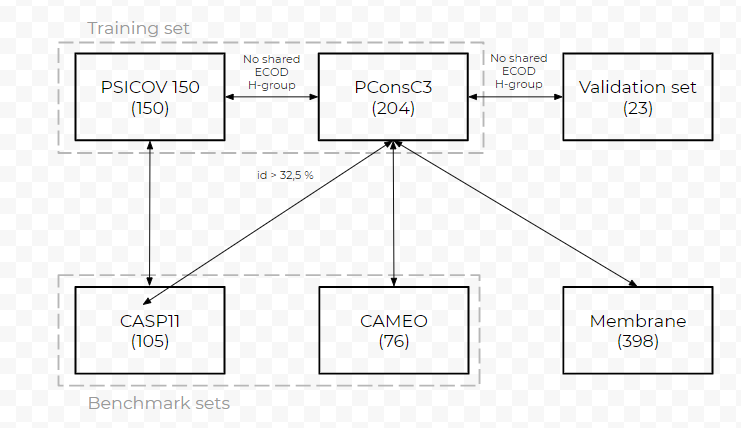
\includegraphics[width=\textwidth, keepaspectratio]{imgs/datasets.png}
         \caption{The different datasets used in this thesis, after homology reduction.}
        \label{homology_reduction}
      \end{center}
    \end{figure}

  \subsection{Feature extraction}

    All protein sequences, structures, multiple sequence alignments present in the three benchmark sets come from the PConsC3 server,
    available at the address \url{http://pconsc3.bioinfo.se/pred/download/} as on the date of 28th December 2018.
    Information available in these datasets is the following:

    \begin{itemize}
      \item Protein sequence in FASTA format
      \item Multiple sequence alignment obtained using HHblits on the corresponding protein family
      \item Native structure in PDB format
      \item PhyCMAP~\cite{PhyCMap} intermediate predictions
      \item plmDCA~\cite{EKEBERG2014341} intermediate predictions
      \item GaussDCA~\cite{10.1371/journal.pone.0092721} intermediate predictions
      \item Predictions made by PConsC3~\cite{Skwark079673} at each layer of the model
      \item CCMPred~\cite{CCMPred} predictions
      \item EVFold~\cite{Sheridan021022} predictions
      \item PSICOV~\cite{doi:10.1093/bioinformatics/btr638} predictions
      \item MetaPSICOV~\cite{MetaPSICOV} predictions
    \end{itemize}

    \subsubsection{Multiple sequence alignments}

        Multiple sequence alignments of the PConsC4's training set are not the same
        as in the original study since they have been retrieved from the
        RaptorX-Property server.

        MSAs for PSICOV150 have been retrieved from the PConsC2 dataset.
        PConsC2 relied on multiple MSAs for predicting contact maps,
        but only the ones generated with HHblits~\cite{HHblits}
        with an e-value of $10^{-4}$
        have been considered in the present thesis.

        MSAs present on the PConsC3 server
        have been created using HHblits
        (version as of the date of 26th February 2016) on the Uniprot20 database
        with an e-value of 1. Parameters have been set in such a way that all
        sequences in each of the database MSAs are aligned.
        These MSAs relate to the three test sets, PConsC3's benchmark set and
        PConsC3's 30 additional proteins.

    \subsubsection{Features}

        The Julia implementation of GaussDCA has been used with default parameters
        on all seven datasets. All other features, including protein length, self-information,
        partial entropies, mutual information, normalized mutual information, etc.
        are computed on-the-fly during the training process.
